\documentclass[10pt]{beamer}\usepackage[]{graphicx}\usepackage[]{color}
%% maxwidth is the original width if it is less than linewidth
%% otherwise use linewidth (to make sure the graphics do not exceed the margin)
\makeatletter
\def\maxwidth{ %
  \ifdim\Gin@nat@width>\linewidth
    \linewidth
  \else
    \Gin@nat@width
  \fi
}
\makeatother

\definecolor{fgcolor}{rgb}{0.196, 0.196, 0.196}
\newcommand{\hlnum}[1]{\textcolor[rgb]{0.063,0.58,0.627}{#1}}%
\newcommand{\hlstr}[1]{\textcolor[rgb]{0.063,0.58,0.627}{#1}}%
\newcommand{\hlcom}[1]{\textcolor[rgb]{0.588,0.588,0.588}{#1}}%
\newcommand{\hlopt}[1]{\textcolor[rgb]{0.196,0.196,0.196}{#1}}%
\newcommand{\hlstd}[1]{\textcolor[rgb]{0.196,0.196,0.196}{#1}}%
\newcommand{\hlkwa}[1]{\textcolor[rgb]{0.231,0.416,0.784}{#1}}%
\newcommand{\hlkwb}[1]{\textcolor[rgb]{0.627,0,0.314}{#1}}%
\newcommand{\hlkwc}[1]{\textcolor[rgb]{0,0.631,0.314}{#1}}%
\newcommand{\hlkwd}[1]{\textcolor[rgb]{0.78,0.227,0.412}{#1}}%
\let\hlipl\hlkwb

\usepackage{framed}
\makeatletter
\newenvironment{kframe}{%
 \def\at@end@of@kframe{}%
 \ifinner\ifhmode%
  \def\at@end@of@kframe{\end{minipage}}%
  \begin{minipage}{\columnwidth}%
 \fi\fi%
 \def\FrameCommand##1{\hskip\@totalleftmargin \hskip-\fboxsep
 \colorbox{shadecolor}{##1}\hskip-\fboxsep
     % There is no \\@totalrightmargin, so:
     \hskip-\linewidth \hskip-\@totalleftmargin \hskip\columnwidth}%
 \MakeFramed {\advance\hsize-\width
   \@totalleftmargin\z@ \linewidth\hsize
   \@setminipage}}%
 {\par\unskip\endMakeFramed%
 \at@end@of@kframe}
\makeatother

\definecolor{shadecolor}{rgb}{.97, .97, .97}
\definecolor{messagecolor}{rgb}{0, 0, 0}
\definecolor{warningcolor}{rgb}{1, 0, 1}
\definecolor{errorcolor}{rgb}{1, 0, 0}
\newenvironment{knitrout}{}{} % an empty environment to be redefined in TeX

\usepackage{alltt}
\usetheme[numbering = fraction, progressbar = frametitle, everytitleformat = regular]{metropolis}

\usepackage{etex} % helps fix \newdimen error which is cause when ctable is loaded with other packages
\usepackage{comment}
\usepackage{ctable}
\usepackage{amsmath,amsthm,amssymb}
\newtheorem{rcode}{R code}[section]
\usepackage{url}

%\usepackage[usenames]{xcolor}
\usepackage{color, colortbl}
\usepackage{tikz}
\usepackage[utf8]{inputenc}
\usepackage[T1]{fontenc}
\usepackage{ae}
%\usepackage{aeguill}

\usetikzlibrary{shapes.geometric, arrows,shapes.symbols,decorations.pathreplacing}
\tikzstyle{startstop} = [rectangle, rounded corners, minimum width=3cm, minimum height=1cm, draw=black, fill=pinkish,text width=3.5cm]
\tikzstyle{startstop2} = [rectangle, rounded corners, minimum width=3cm, minimum height=1cm, draw=black, fill=background,text width=4.5cm]
\tikzstyle{startstop3} = [rectangle, rounded corners, minimum width=3cm, minimum height=1cm, draw=black, fill=beige,text width=3.0cm]
\tikzstyle{startstop4} = [rectangle, rounded corners, minimum width=3cm, minimum height=1cm, draw=black, fill=pinkish,text width=4.5cm]
\tikzstyle{io} = [trapezium, trapezium left angle=70, trapezium right angle=110, minimum width=2cm, minimum height=1cm, text centered, draw=black, fill=blue!30,text width=1.5cm]
\tikzstyle{process} = [rectangle, minimum width=1cm, minimum height=1cm, text centered, draw=black, fill=orange!30,text width=2cm]
\tikzstyle{decision} = [diamond, minimum width=2cm, minimum height=1cm, text centered, draw=black, fill=green!30]
\tikzstyle{arrow} = [thick,->,>=stealth]
\tikzstyle{both} = [thick,<->,>=stealth, red]

\tikzset{myshade/.style={minimum size=.4cm,shading=radial,inner color=white,outer color={#1!90!gray}}}
\newcommand\mycirc[1][]{\tikz\node[circle,myshade=#1]{};}
\newcommand\myrect[1][]{\tikz\node[rectangle,myshade=#1]{};}
\newcommand\mystar[1][]{\tikz\node[star,star points=15,star point height=2pt,myshade=#1]{};}
\newcommand\mydiamond[1][]{\tikz\node[diamond,myshade=#1]{};}
\newcommand\myellipse[1][]{\tikz\node[ellipse,myshade=#1]{};}
\newcommand\mykite[1][]{\tikz\node[kite,myshade=#1]{};}
\newcommand\mydart[1][]{\tikz\node[dart,myshade=#1]{};}
\newcommand\mycloud[1][]{\tikz\node[cloud,myshade=#1]{};}

%\usepackage{subcaption}
\usepackage{subfig}
%\usepackage{caption}


\usepackage[]{hyperref}
\hypersetup{
    unicode=false,          
    pdftoolbar=true,        
    pdfmenubar=true,        
    pdffitwindow=false,     % window fit to page when opened
    pdfstartview={FitH},    % fits the width of the page to the window
    pdftitle={useR Montreal August 12, 2015},    % title
    pdfauthor={Sahir Rai Bhatnagar},     % author
    pdfsubject={Subject},   % subject of the document
    pdfcreator={Sahir Rai Bhatnagar},   % creator of the document
    pdfproducer={Sahir Rai Bhatnagar}, % producer of the document
    pdfkeywords={}, % list of keywords
    pdfnewwindow=true,      % links in new window
    colorlinks=true,       % false: boxed links; true: colored links
    linkcolor=red,          % color of internal links (change box color with linkbordercolor)
    citecolor=blue,        % color of links to bibliography
    filecolor=black,      % color of file links
    urlcolor=cyan           % color of external links
}

%\RequirePackage{color}

% define a bunch of colors
\definecolor{gray}{RGB}{110,110,110}
\definecolor{darkgray}{RGB}{100,100,100}
\definecolor{lightgray}{RGB}{200,200,200}
\definecolor{turquoise}{RGB}{81,193,188}
\definecolor{tomato}{RGB}{255,136,136}
\definecolor{mandarina}{RGB}{229,169,25}
\definecolor{foreground}{RGB}{81,141,193}
\definecolor{background}{RGB}{246,244,240}
\definecolor{highlight}{RGB}{229,169,25}
\definecolor{lowlight}{RGB}{200,200,200}
\definecolor{beige}{RGB}{255,255,240}
\definecolor{pinkish}{RGB}{255,223,247}
%\definecolor{aliceblue}{rgb}{0.94, 0.97, 1.0}
%\definecolor{antiflashwhite}{rgb}{0.95, 0.95, 0.96}

% some convenient commands
\newcommand{\code}[1]{\texttt{#1}}
\newcommand{\high}[1]{\textcolor{highlight}{#1}}
\newcommand{\low}[1]{\textcolor{lowlight}{#1}}
\newcommand{\highcode}[1]{\textcolor{highlight}{\texttt{#1}}}

%\setbeamercolor{block body}{bg=beige}
\setbeamertemplate{theorems}[numbered] % so that you can number the R code theorem environments

%\setbeamercovered{highly dynamic}

\newcounter{saveenumi}
\newcommand{\seti}{\setcounter{saveenumi}{\value{enumi}}}
\newcommand{\conti}{\setcounter{enumi}{\value{saveenumi}}}


%\title{Introduction to } % load mtheme
% define title
\date{\today}
\author{Sahir Bhatnagar} % define date
% define author
\institute{McGill Univeristy}

\title{An Introduction to \texttt{knitr} and \texttt{RMarkdown}}
\subtitle{\href{https://github.com/sahirbhatnagar/knitr-tutorial}{https://github.com/sahirbhatnagar/knitr-tutorial}}
\IfFileExists{upquote.sty}{\usepackage{upquote}}{}
\begin{document}





\maketitle % define institute


%\section{Acknowledments}

\begin{frame}{Acknowledgements}
% \hspace*{-1.9cm}\parbox[t]{\textwidth}
%\frametitle{Acknowledgements}
\begin{columns}[c] % The "c" option specifies centered vertical alignment while the "t" option is used for top vertical alignment

\column{.45\textwidth} % Left column and width

\begin{itemize}
%\scriptsize
\item Toby, Matthieu, Vaughn, Ary
\item \href{http://turgeonmaxime.github.io/}{Maxime Turgeon} (Windows)
\item \href{https://www.researchgate.net/profile/Kevin_Mcgregor2}{Kevin McGregor} (Mac)
\item Greg Voisin
\item \href{http://www-cs-faculty.stanford.edu/~uno/}{Don Knuth} (\TeX)
\item \href{http://www.statistik.lmu.de/~leisch/}{Friedrich Leisch} (Sweave)
\item \href{http://yihui.name/knitr/}{Yihui Xie} (knitr)
\item \href{http://daringfireball.net/projects/markdown/}{John Gruber} (Markdown)
\item \href{http://pandoc.org/}{John MacFarlane} (Pandoc)
\item You
\end{itemize}

\column{.45\textwidth} % Right column and width
\begin{figure}

\includegraphics[width=0.8\columnwidth]{mtluser.png}\\[5mm]

\includegraphics[width=0.8\columnwidth]{notman.png}\\[5mm]

\includegraphics[width=0.8\columnwidth]{revo.png}
\end{figure}

\end{columns}
\end{frame}


\begin{frame}{Disclaimer \#1}
\begin{figure}

\includegraphics[width=0.8\columnwidth]{rstudio.png}\\[5mm]

\includegraphics[width=0.2\columnwidth]{rlogo.png}\\[5mm]

\includegraphics[width=0.2\columnwidth]{LaTeX_logo.png}
\end{figure}

\textit{I don't work for, nor am I an author of any of these packages. I'm just a messenger.}

\end{frame}

\begin{frame}{Disclaimer \#2}

\begin{itemize}
\item Material for this tutorial comes from many sources. For a complete list see:  \href{https://github.com/sahirbhatnagar/knitr-tutorial}{https://github.com/sahirbhatnagar/knitr-tutorial}
\item Alot of the content in these slides are based on these two books
\end{itemize}

\begin{columns}[c] % The "c" option specifies centered vertical alignment while the "t" option is used for top vertical alignment
\column{.45\textwidth} % Left column and width
\begin{figure}
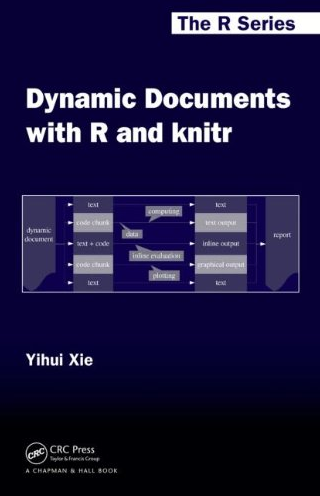
\includegraphics[width=0.6\columnwidth]{yihui.png}
\end{figure}

\column{.45\textwidth} % Right column and width
\begin{figure}
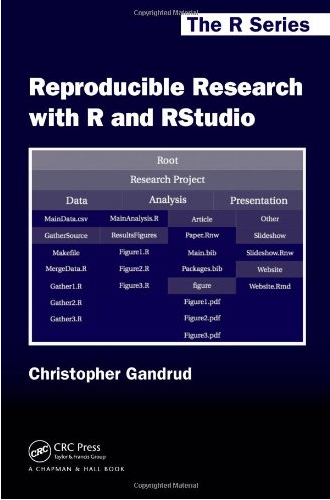
\includegraphics[width=0.6\columnwidth]{chris.png}
\end{figure}
\end{columns}

\end{frame}

\begin{frame}{Objectives for today}
% \hspace*{-1.9cm}\parbox[t]{\textwidth}
%\frametitle{Acknowledgements}
\begin{columns}[c] % The "c" option specifies centered vertical alignment while the "t" option is used for top vertical alignment

\column{.45\textwidth} % Left column and width

\begin{itemize}
%\scriptsize
\item Create a reproducible document (\code{pdf, html})
\end{itemize}
\pause 
\column{.45\textwidth} % Right column and width
\begin{figure}
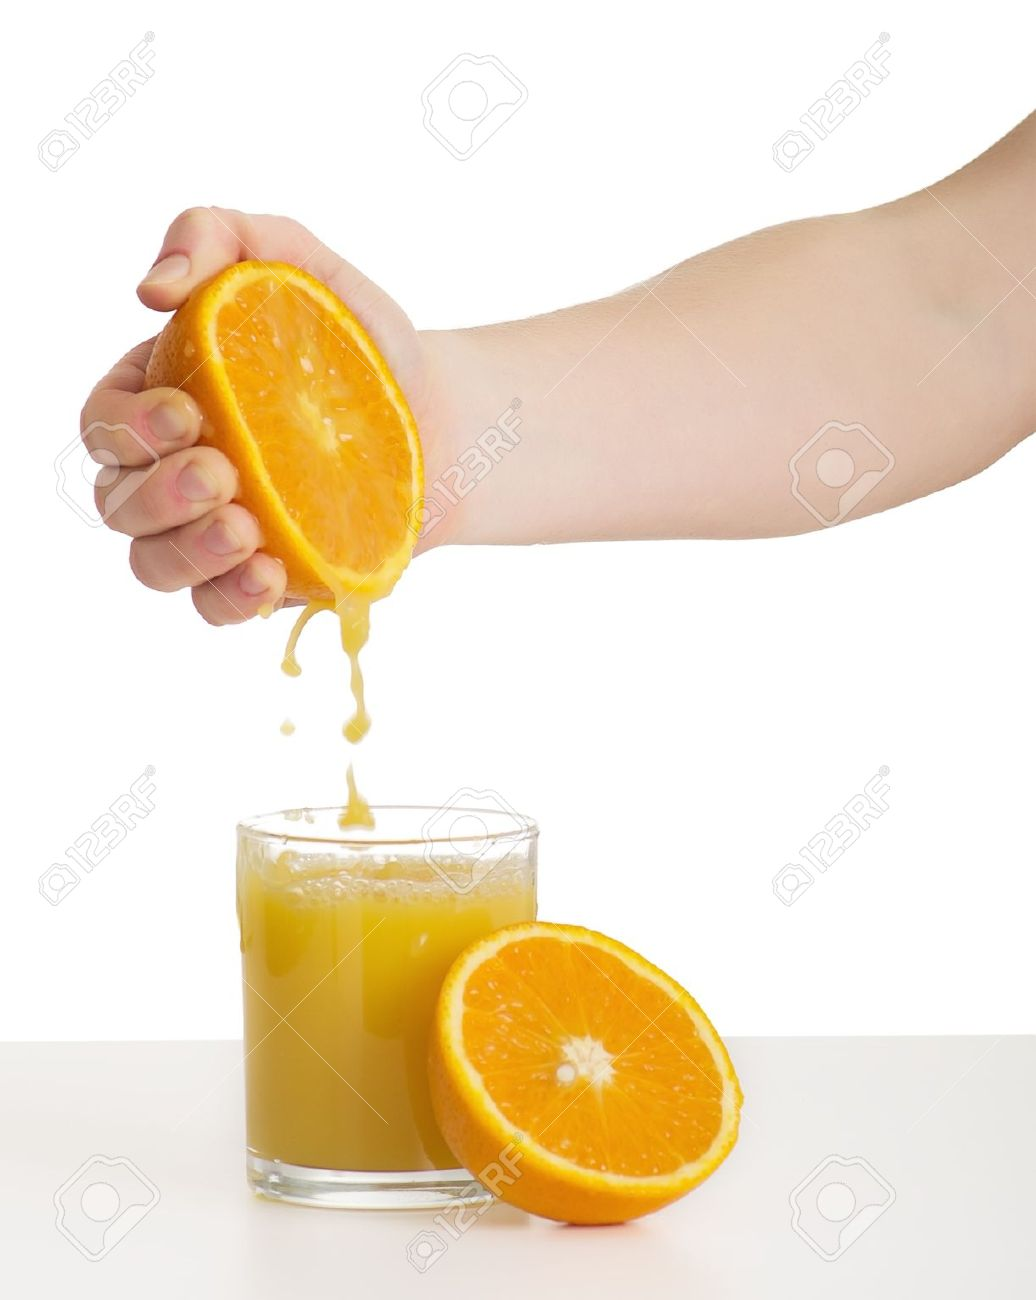
\includegraphics[width=0.8\columnwidth]{./juice}
\end{figure}

\end{columns}
\end{frame}


\begin{frame}{C'est parti}
%\hspace*{-1.5cm}\parbox[t]{\textwidth}{
\begin{center}
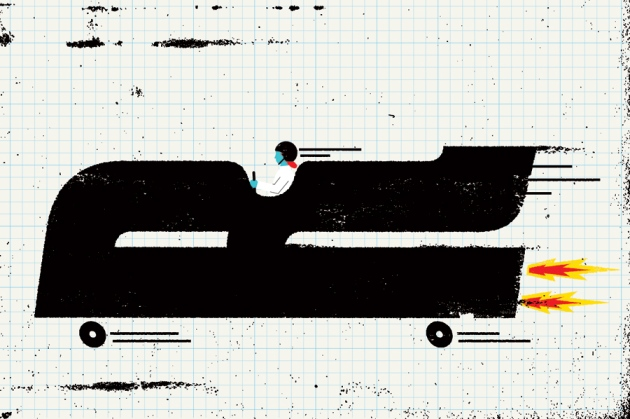
\includegraphics[scale=0.51]{introR.jpg}
\end{center}
%}
\end{frame}

\section{What?}


\begin{frame}{What is needed for Reproducible research?}
\def\firstcircle{(0,0) circle (1.5cm)}
\def\secondcircle{(45:2cm) circle (1.5cm)}
\def\thirdcircle{(0:2cm) circle (1.5cm)}
% Now we can draw the sets:
\begin{center}
\begin{tikzpicture}
    \draw \firstcircle node[below] {code};
    \draw \secondcircle node [above] {data};
    \draw \thirdcircle node [below] {text};

    % Now we want to highlight the intersection of the first and the
    % second circle:

    %\begin{scope}
    %  \clip \firstcircle;
    %  \fill[red] \secondcircle;
    %\end{scope}

    % Next, we want the highlight the intersection of all three circles:

    \begin{scope}
      \clip \firstcircle;
      \clip \secondcircle;
      \fill[green] \thirdcircle;
    \end{scope}
\end{tikzpicture}
\end{center}
\end{frame}

\section{Why?}

\begin{frame}
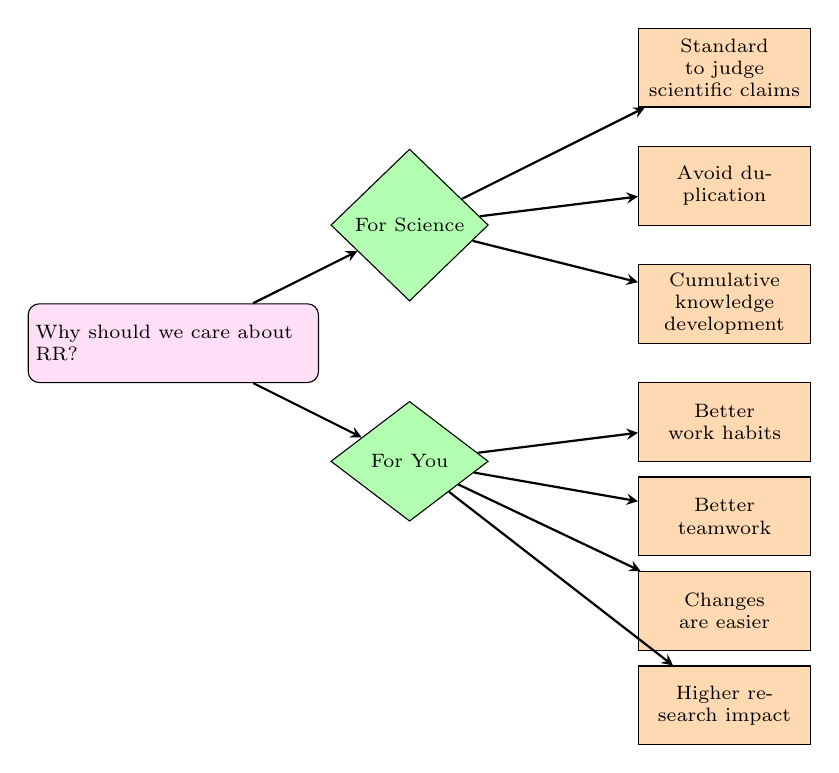
\begin{tikzpicture}
\scriptsize
\node (expr) [startstop] {Why should we care about RR?};
\node (science) [decision, right of=expr, xshift=2cm, yshift=1.5cm] {For Science};
\draw [arrow] (expr) -- (science);
\node (stan) [process, right of=science, xshift=3cm, yshift=2cm] {Standard to judge scientific claims};
\node (dupli) [process, right of=science, xshift=3cm, yshift=0.5cm] {Avoid duplication};
\node (know) [process, right of=science, xshift=3cm, yshift=-1cm] {Cumulative knowledge development};
\draw [arrow] (science) -- (stan);
\draw [arrow] (science) -- (dupli);
\draw [arrow] (science) -- (know);
\pause \node (you) [decision, right of=expr, xshift=2cm, yshift=-1.5cm] {For You};
\draw [arrow] (expr) -- (you);
\node (work) [process, right of=you, xshift=3cm, yshift=0.5cm] {Better work habits};
\node (team) [process, right of=you, xshift=3cm, yshift=-0.7cm] {Better teamwork};
\node (change) [process, right of=you, xshift=3cm, yshift=-1.9cm] {Changes are easier};
\node (soft) [process, right of=you, xshift=3cm, yshift=-3.1cm] {Higher research impact};
\draw [arrow] (you) -- (work);
\draw [arrow] (you) -- (team);
\draw [arrow] (you) -- (change);
\draw [arrow] (you) -- (soft);
\end{tikzpicture}
\end{frame}

\section{001-motivating-example}

\begin{frame}{A Motivating Example}
\textit{Demonstrate:} \href{https://github.com/sahirbhatnagar/knitr-tutorial/tree/master/001-motivating-example}{001-motivating-example}\\
\end{frame}



\section{How?}

\begin{frame}{Tools for Reproducible Research}

\begin{block}{Free and Open Source Software}
\begin{itemize}
\item \texttt{RStudio}: Creating, managing, compiling documents
\item \LaTeX: Markup language for typesetting a pdf
\item Markdown: Markup language for typesetting an html
\item \texttt{R}: Statistical analysis language
\item \texttt{knitr}: Integrate \LaTeX and \texttt{R} code. Based on Prof. Friedrich Leisch's \href{https://www.statistik.lmu.de/~leisch/Sweave/}{\texttt{Sweave}}
\end{itemize}
\end{block}
\end{frame}

%\begin{frame}\frametitle{RStudio: Integrated Development Environment (IDE)}
%\begin{figure}[h!]
%\centering
%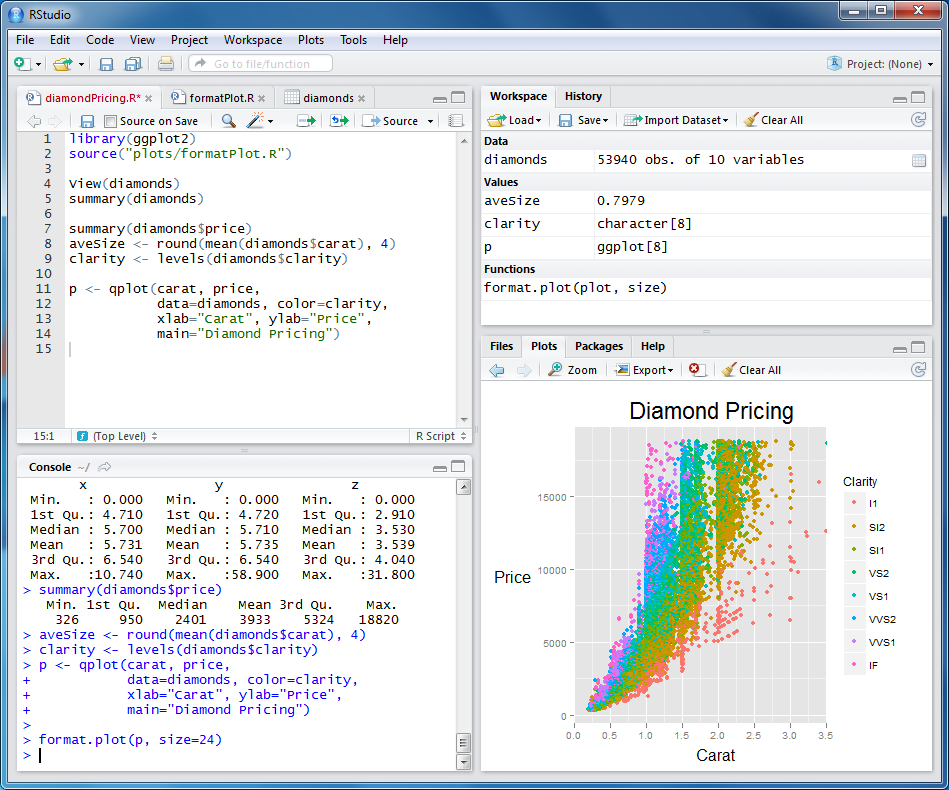
\includegraphics[scale=0.25, keepaspectratio]{./RStudio-Screenshot}
%\end{figure}
%\textit{Demonstrate:} Explore \texttt{RStudio} 
%\end{frame}


\section{\texttt{knitr}}

\begin{frame}{What \texttt{knitr} does}
\textbf{\LaTeX} example:

\begin{center}
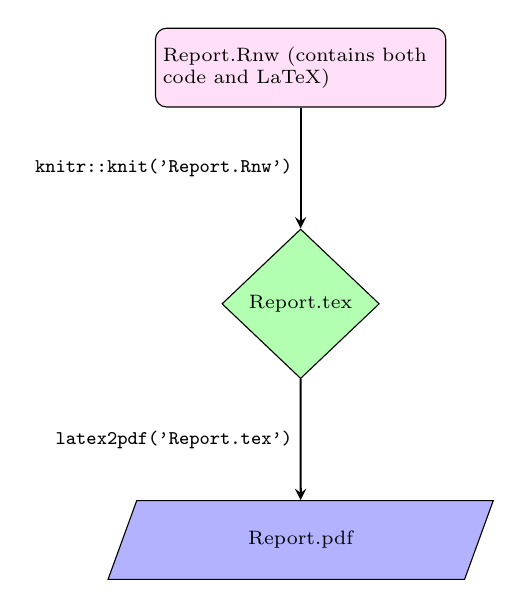
\begin{tikzpicture}
\scriptsize
\node (expr) [startstop] {Report.Rnw (contains both code and LaTeX)};
\node (science) [decision, below of=expr, xshift=0cm, yshift=-2cm] {Report.tex};
\draw [arrow] (expr) -- node[anchor=east]{\texttt{knitr::knit('Report.Rnw')}} (science);
\pause \node (pdf) [io, below of=science, xshift=0cm, yshift=-2cm] {Report.pdf};
\draw [arrow] (science) -- node[anchor=east]{\texttt{latex2pdf('Report.tex')}} (pdf);
\end{tikzpicture}
\end{center}
\end{frame}


\begin{frame}\frametitle{Compiling a \texttt{.Rnw} document}

\begin{block}{The two steps on previous slide can be executed in one command:}
\[ \textrm{\texttt{knitr::knit2pdf()}} \]
\end{block}

or in \texttt{RStudio}:
\begin{figure}[h!]
\centering
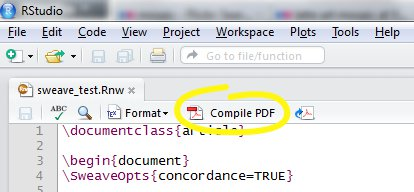
\includegraphics[scale=0.5, keepaspectratio]{./Compile-pdf.jpg}
\end{figure}
%\textit{Demonstrate:} Explore \texttt{RStudio}, projects and \texttt{.Rprofile}
\end{frame}

\begin{frame}\frametitle{Incorporating \texttt{R} code}

\begin{itemize}
\item Insert \texttt{R} code in a \textbf{Code Chunk} starting with $$ << \quad >>= $$
and ending with \begin{center}
{@}
\end{center}
\end{itemize}

In \texttt{RStudio}:
\begin{figure}[h!]
\centering
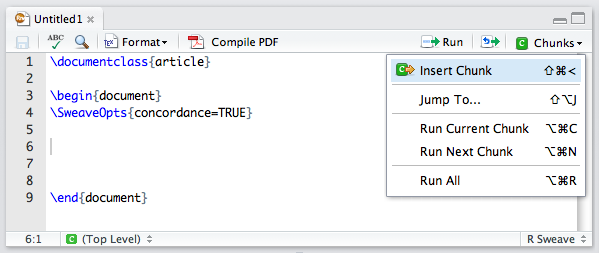
\includegraphics[scale=0.35, keepaspectratio]{./sweave_chunk}
\end{figure}
%\textit{Demonstrate:} Explore \texttt{RStudio}, projects and \texttt{.Rprofile}
\end{frame}

\begin{frame}[fragile]{Example 1: Show code and results}
\begin{knitrout}
\definecolor{shadecolor}{rgb}{1, 1, 1}\color{fgcolor}\begin{kframe}
\begin{verbatim}
<<example-code-chunk-name, echo=TRUE>>=
x <- rnorm(50)
mean(x)
@
\end{verbatim}
\end{kframe}
\end{knitrout}
produces
\begin{knitrout}
\definecolor{shadecolor}{rgb}{1, 1, 1}\color{fgcolor}\begin{kframe}
\begin{alltt}
\hlstd{x} \hlkwb{<-} \hlkwd{rnorm}\hlstd{(}\hlnum{50}\hlstd{)}
\hlkwd{mean}\hlstd{(x)}
\end{alltt}
\begin{verbatim}
## [1] 0.12
\end{verbatim}
\end{kframe}
\end{knitrout}
\end{frame}


\begin{frame}[fragile]{Example 2: Tidy code}
\begin{knitrout}
\definecolor{shadecolor}{rgb}{1, 1, 1}\color{fgcolor}\begin{kframe}
\begin{verbatim}
<<example-code-chunk-name2, echo=TRUE, tidy=TRUE>>=
for(i in 1:5){ print(i+3)}
@
\end{verbatim}
\end{kframe}
\end{knitrout}
produces
\begin{knitrout}
\definecolor{shadecolor}{rgb}{1, 1, 1}\color{fgcolor}\begin{kframe}
\begin{alltt}
\hlkwa{for} \hlstd{(i} \hlkwa{in} \hlnum{1}\hlopt{:}\hlnum{5}\hlstd{) \{}
    \hlkwd{print}\hlstd{(i} \hlopt{+} \hlnum{3}\hlstd{)}
\hlstd{\}}
\end{alltt}
\begin{verbatim}
## [1] 4
## [1] 5
## [1] 6
## [1] 7
## [1] 8
\end{verbatim}
\end{kframe}
\end{knitrout}

\end{frame}


\begin{frame}[fragile]{Example 2.2: don't show code}
\begin{knitrout}
\definecolor{shadecolor}{rgb}{1, 1, 1}\color{fgcolor}\begin{kframe}
\begin{verbatim}
<<example-code-chunk-name3, echo=FALSE>>=
for(i in 1:5){ print(i+3)}
@
\end{verbatim}
\end{kframe}
\end{knitrout}
produces
\begin{knitrout}
\definecolor{shadecolor}{rgb}{1, 1, 1}\color{fgcolor}\begin{kframe}
\begin{verbatim}
## [1] 4
## [1] 5
## [1] 6
## [1] 7
## [1] 8
\end{verbatim}
\end{kframe}
\end{knitrout}

\end{frame}


\begin{frame}[fragile]{Example 2.3: don't evaluate and don't show the code}
\begin{knitrout}
\definecolor{shadecolor}{rgb}{1, 1, 1}\color{fgcolor}\begin{kframe}
\begin{verbatim}
<<example-code-chunk-name4, echo=FALSE, eval=FALSE>>=
for(i in 1:5){ print(i+3)}
@
\end{verbatim}
\end{kframe}
\end{knitrout}
produces


%\textit{Demonstrate:} Try it yourself
\end{frame}



\begin{frame}[fragile]{\texttt{R} output within the text}
\begin{itemize}
\item Include \texttt{R} output within the text
\item We can do that with ``S-expressions'' using the command \textbackslash \texttt{Sexpr}\{$\ldots$\}
\end{itemize}
\vspace{1cm}

\textbf{Example:} \vspace{0.3cm}

The iris dataset has \textbackslash \texttt{Sexpr}\{\texttt{nrow(iris)}\} rows and \textbackslash \texttt{Sexpr}\{\texttt{ncol(iris)}\} columns
\vspace{0.5cm}

produces \vspace{0.5cm}

The iris dataset has 150 rows and 5 columns


\end{frame}


\begin{frame}[fragile]
\frametitle{Include a Figure}
\scriptsize
\begin{knitrout}
\definecolor{shadecolor}{rgb}{1, 1, 1}\color{fgcolor}\begin{kframe}
\begin{verbatim}
<<fig.ex, fig.cap='Linear Regression',fig.height=3,fig.width=3>>=
plot(mtcars[ , c('disp','mpg')])
fit <- lm(mpg ~ disp , data = mtcars)
abline(fit,lwd=2)
@
\end{verbatim}
\end{kframe}
\end{knitrout}
\begin{knitrout}
\definecolor{shadecolor}{rgb}{1, 1, 1}\color{fgcolor}\begin{figure}

{\centering 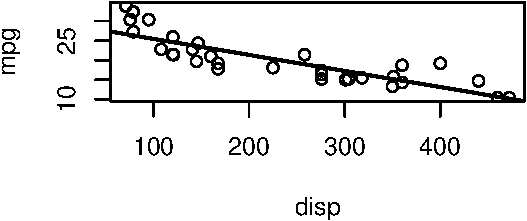
\includegraphics[width=\maxwidth]{figure/slr7-1} 

}

\caption[Linear regression]{Linear regression}\label{fig:slr7}
\end{figure}


\end{knitrout}
\end{frame}



\begin{frame}[fragile]
\frametitle{Include a Table}
\scriptsize
\begin{knitrout}
\definecolor{shadecolor}{rgb}{1, 1, 1}\color{fgcolor}\begin{kframe}
\begin{verbatim}
<<table.ex, results='asis'>>=
library(xtable)
tab <- xtable(iris[1:5,1:5],caption='Sample of Iris data')
print(tab, include.rownames=FALSE)
@
\end{verbatim}
\end{kframe}
\end{knitrout}
\begin{kframe}
\begin{alltt}
\hlkwd{library}\hlstd{(xtable)}
\hlstd{tab} \hlkwb{<-} \hlkwd{xtable}\hlstd{(iris[}\hlnum{1}\hlopt{:}\hlnum{5}\hlstd{,}\hlnum{1}\hlopt{:}\hlnum{5}\hlstd{],} \hlkwc{caption} \hlstd{=} \hlstr{'Sample of Iris data'}\hlstd{)}
\hlkwd{print}\hlstd{(tab,} \hlkwc{include.rownames} \hlstd{= F)}
\end{alltt}
\end{kframe}% latex table generated in R 3.4.4 by xtable 1.8-2 package
% Tue Jun 26 23:12:50 2018
\begin{table}[ht]
\centering
\begin{tabular}{rrrrl}
  \hline
Sepal.Length & Sepal.Width & Petal.Length & Petal.Width & Species \\ 
  \hline
5.10 & 3.50 & 1.40 & 0.20 & setosa \\ 
  4.90 & 3.00 & 1.40 & 0.20 & setosa \\ 
  4.70 & 3.20 & 1.30 & 0.20 & setosa \\ 
  4.60 & 3.10 & 1.50 & 0.20 & setosa \\ 
  5.00 & 3.60 & 1.40 & 0.20 & setosa \\ 
   \hline
\end{tabular}
\caption{Sample of Iris data} 
\end{table}

\end{frame}


\begin{comment}
\section{Details}

\subsection{Code Chunks}

\begin{frame}{A selection of \texttt{knitr} code chunk options}
content...
\end{frame}


\begin{frame}{Set global chunk options}
content...
\end{frame}


\begin{frame}{Option Aliases}
see page 109 yihui
\end{frame}


\begin{frame}{Option Templates}
see page 110 yihui
\end{frame}

\begin{frame}{Chunk References}
see page 79 yihui
\end{frame}


\begin{frame}{Code in Appendix}
see page 110 yihui
\end{frame}



\subsection{Hooks}
\begin{frame}{A selection of \texttt{knitr} code chunk options}
content...
\end{frame}


\subsection{Child Documents}
\begin{frame}{A selection of \texttt{knitr} code chunk options}
see 83
\end{frame}



\subsection{Custom Environments}
\begin{frame}{Example Environment}
see 120
\end{frame}
\end{comment}

\begin{comment}
\section{Examples}

\subsection{002-minimum-working-example}

\begin{frame}{Minimum Working Example}
\href{https://github.com/sahirbhatnagar/knitr-tutorial/tree/master/002-minimum-working-example}{https://github.com/sahirbhatnagar/knitr-tutorial/tree/master/002-minimum-working-example}
\end{frame}


\subsection{003-model-output}

\begin{frame}{Extracting output from Regression Models}
\href{https://github.com/sahirbhatnagar/knitr-tutorial/tree/master/003-model-output}{https://github.com/sahirbhatnagar/knitr-tutorial/tree/master/003-model-output}
\end{frame}


\subsection{004-figures}

\begin{frame}{Figures}
\href{https://github.com/sahirbhatnagar/knitr-tutorial/tree/master/004-figures}{https://github.com/sahirbhatnagar/knitr-tutorial/tree/master/004-figures}
\end{frame}


\subsection{005-beamer-presentation}

\begin{frame}{Beamer Presentations}
\href{https://github.com/sahirbhatnagar/knitr-tutorial/tree/master/005-beamer-presentation}{https://github.com/sahirbhatnagar/knitr-tutorial/tree/master/005-beamer-presentation}
\end{frame}


\subsection{006-sensitivity-analysis-one-parameter}

\begin{frame}{Changing one Parameter in an Analysis}
\href{https://github.com/sahirbhatnagar/knitr-tutorial/tree/master/006-sensitivity-analysis-one-parameter}{https://github.com/sahirbhatnagar/knitr-tutorial/tree/master/006-sensitivity-analysis-one-parameter}
\end{frame}

\subsection{007-sensitivity-analysis-many-parameters}

\begin{frame}{Changing Many Parameters in an Analysis}
\href{https://github.com/sahirbhatnagar/knitr-tutorial/tree/master/007-sensitivity-analysis-many-parameters}{https://github.com/sahirbhatnagar/knitr-tutorial/tree/master/007-sensitivity-analysis-many-parameters}
\end{frame}


\subsection{008-large-documents}

\begin{frame}{Large Documents}
\href{https://github.com/sahirbhatnagar/knitr-tutorial/tree/master/008-large-documents}{https://github.com/sahirbhatnagar/knitr-tutorial/tree/master/008-large-documents}
\end{frame}

\subsection{009-rmarkdown}

\begin{frame}{HTML Reports}
\href{https://github.com/sahirbhatnagar/knitr-tutorial/tree/master/009-rmarkdown}{https://github.com/sahirbhatnagar/knitr-tutorial/tree/master/009-rmarkdown}
\end{frame}

\subsection{010-rmarkdown-presentation}

\begin{frame}{HTML Presentations}
\href{https://github.com/sahirbhatnagar/knitr-tutorial/tree/master/010-rmarkdown-presentation}{https://github.com/sahirbhatnagar/knitr-tutorial/tree/master/010-rmarkdown-presentation}
\end{frame}
\end{comment}


\section{RMarkdown}

\begin{frame}{Markdown: HTML without knowing HTML}
\begin{center}
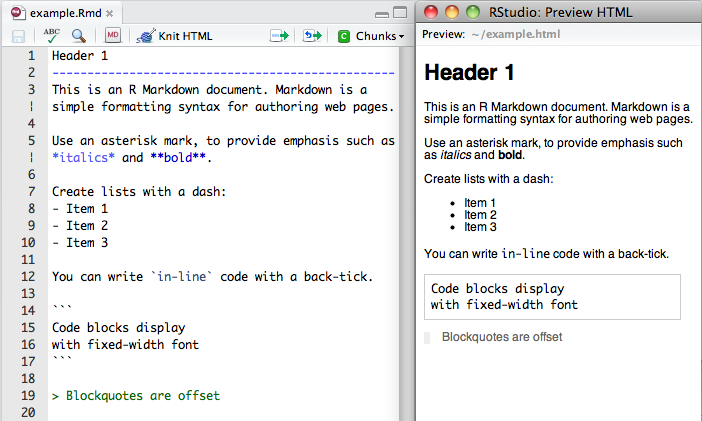
\includegraphics[scale=0.45, keepaspectratio]{markdown}
\end{center}
\end{frame}

\begin{frame}{R + Markdown = RMarkdown}
\begin{center}
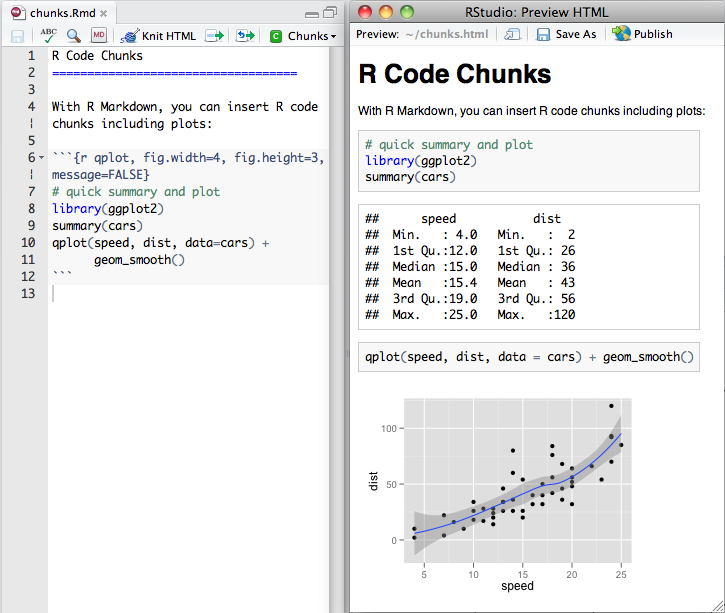
\includegraphics[scale=0.36, keepaspectratio]{rmarkdown}
\end{center}
\end{frame}

\begin{frame}{What \texttt{rmarkdown} does}
\textbf{\code{RMarkdown}} example:

\begin{center}
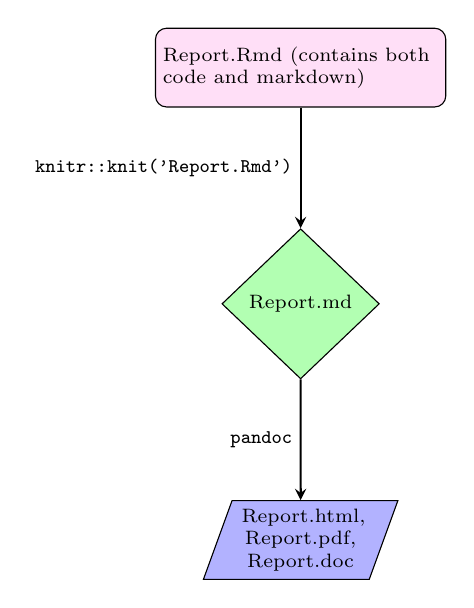
\begin{tikzpicture}
\scriptsize
\node (expr) [startstop] {Report.Rmd (contains both code and markdown)};
\node (science) [decision, below of=expr, xshift=0cm, yshift=-2cm] {Report.md};
\draw [arrow] (expr) -- node[anchor=east]{\texttt{knitr::knit('Report.Rmd')}} (science);
\pause \node (pdf) [io, below of=science, xshift=0cm, yshift=-2cm] {Report.html, Report.pdf, Report.doc};
\draw [arrow] (science) -- node[anchor=east]{\texttt{pandoc}} (pdf);
\end{tikzpicture}
\end{center}
\end{frame}


\begin{frame}\frametitle{Compiling a \texttt{.Rmd} document}

\begin{block}{The two steps on previous slide can be executed in one command:}
\[ \textrm{\texttt{rmarkdown::render()}} \]
\end{block}

or in \texttt{RStudio}:
\begin{figure}[h!]
\centering
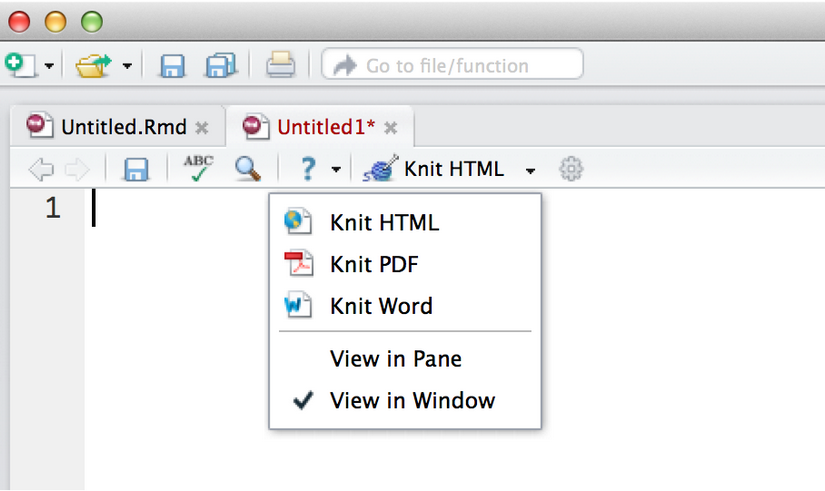
\includegraphics[scale=0.21, keepaspectratio]{rmddrop.png}
\end{figure}
%\textit{Demonstrate:} Explore \texttt{RStudio}, projects and \texttt{.Rprofile}
\end{frame}


\section{Final Remarks}

\begin{frame}{How to choose between \LaTeX\mbox{ }and Markdown ?}
 %\hspace*{-1.9cm}\parbox[t]{\textwidth}{
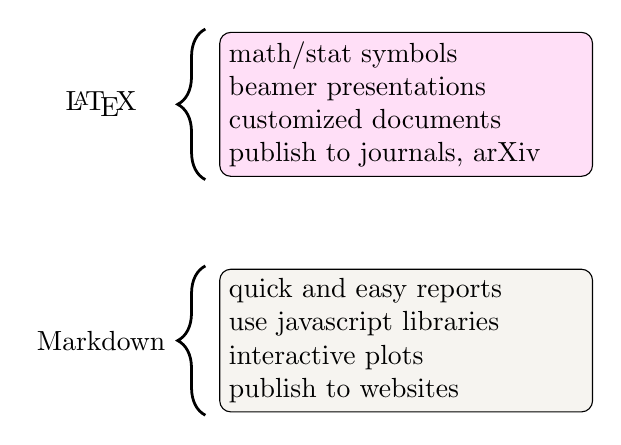
\begin{tikzpicture}
\node (expr) [startstop4] {math/stat symbols \textcolor{pinkish}{tecccccc}
beamer presentations \textcolor{pinkish}{teccccc}
customized documents \textcolor{pinkish}{tecccc}
publish to journals, arXiv 
%\code{getwd()}\textcolor{pinkish}{teccc}
%\code{rm()}\textcolor{pinkish}{tevvvvvvv}
 };
\node (fat) [startstop2, below of=expr, xshift=-.0cm, yshift=-2.0cm] {quick and easy reports\textcolor{background}{tkkk} 
use javascript libraries \textcolor{background}{tekkt}
interactive plots \textcolor{background}{texkkkkjjt}
publish to websites};
%\node (script) [startstop3, below of=fat, xshift=.1cm, yshift=-1.5cm] {
%\code{read.table()}
%\code{write.table()}
%\code{load()}
%\code{save()}\textcolor{beige}{text}
%\code{source()}};
\draw[decoration={brace,raise=5pt, amplitude=10pt},decorate,line width=1pt] 
  ([yshift=-1pt]expr.south west) -- ([yshift=1pt]expr.north west) node [black,midway,xshift=-1.5cm] 
{ \LaTeX};
\draw[decoration={brace,raise=5pt,amplitude=10pt},decorate,line width=1pt] 
  ([yshift=-1pt]fat.south west) -- ([yshift=1pt]fat.north west) node [black,midway,xshift=-1.5cm] 
{Markdown};
%\draw[decoration={brace,raise=5pt,amplitude=10pt},decorate,line width=1pt] 
%  ([yshift=-1pt]script.south west) -- ([yshift=1pt]script.north west) node [black,midway,xshift=-3cm] 
{\footnotesize Accéder les données et scripts R};
\end{tikzpicture}
%}
\end{frame}



\begin{frame}
\begin{figure}[h!]
\centering
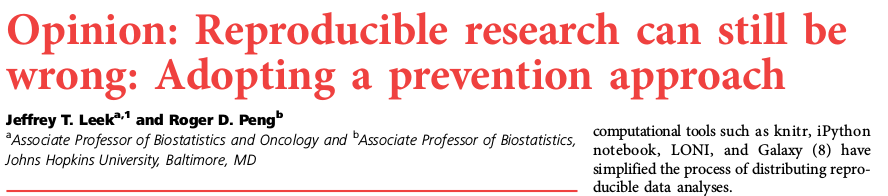
\includegraphics[scale=0.30, keepaspectratio]{./leek}
\end{figure}
\end{frame}

\begin{frame}
\frametitle{Always Remember ...}

\[ \textrm{Reproducibility} \propto \frac{1}{\textrm{copy paste}}  \]


\end{frame}


\begin{frame}{Is the juice worth the squeeze?}
\begin{figure}[h!]
\centering
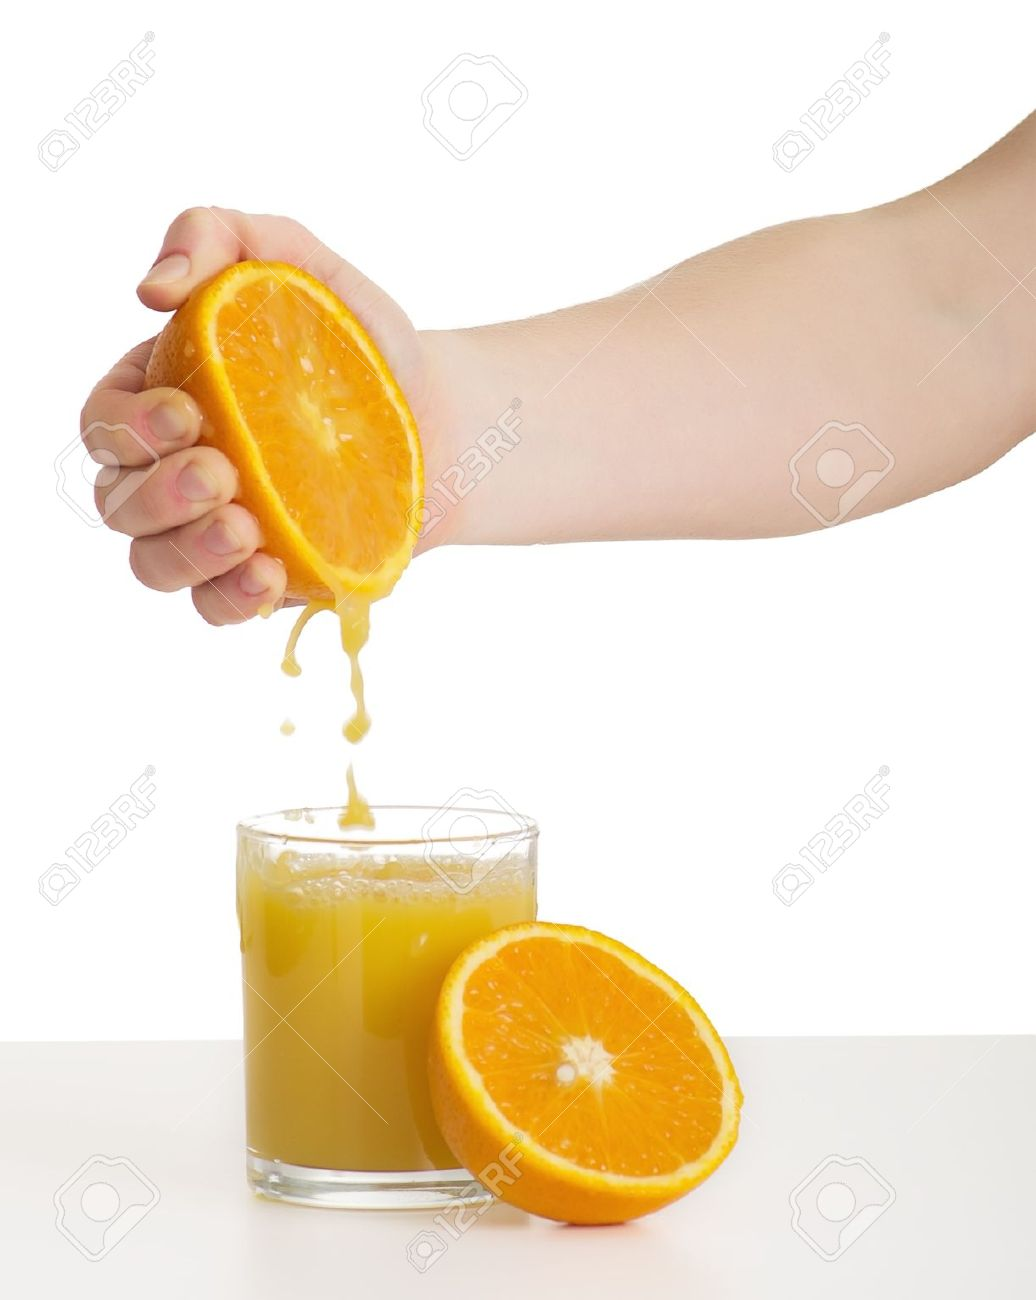
\includegraphics[scale=0.40, keepaspectratio]{./juice}
\end{figure}
\end{frame}

\begin{frame}[fragile]{Session Info}
\begin{itemize}\raggedright
  \item R version 3.4.4 (2018-03-15), \verb|x86_64-pc-linux-gnu|
  \item Running under: \verb|Ubuntu 16.04.4 LTS|
  \item Matrix products: default
  \item BLAS: \verb|/usr/lib/openblas-base/libblas.so.3|
  \item LAPACK: \verb|/usr/lib/libopenblasp-r0.2.18.so|
  \item Base packages: base, datasets, graphics, grDevices, methods,
    stats, utils
  \item Other packages: data.table~1.10.4-3, dplyr~0.7.5,
    ggplot2~2.2.1.9000, knitr~1.20, xtable~1.8-2
  \item Loaded via a namespace (and not attached): assertthat~0.2.0,
    bindr~0.1.1, bindrcpp~0.2.2, colorspace~1.3-2, compiler~3.4.4,
    evaluate~0.10.1, formatR~1.5, glue~1.2.0, grid~3.4.4,
    gtable~0.2.0, highr~0.7, lazyeval~0.2.1, magrittr~1.5,
    munsell~0.4.3, pillar~1.2.3, pkgconfig~2.0.1, plyr~1.8.4,
    purrr~0.2.5, R6~2.2.2, Rcpp~0.12.17, rlang~0.2.0.9001,
    scales~0.5.0.9000, stringi~1.2.3, stringr~1.3.1, tibble~1.4.2,
    tidyselect~0.2.4, tools~3.4.4, withr~2.1.2
\end{itemize}

Slides made with Beamer \href{https://github.com/matze/mtheme}{mtheme}
\end{frame}



\end{document}

